% !TeX root = ../tesis.tex

\chapter{Esparcimiento de luz por partículas}
\label{chapter:theory}

\vspace*{7em}

It is recommended to write a summary about the contents of this chapter as an introduction to them. 


\section{Fundamentos}
\label{section:basics}

La electrodinámica clásica es descrita mediante la fuerza de Lorentz y las ecuaciones de Maxwell \cite{griffithsIntroductionElectrodynamics2023}. En el sistema internacional de unidades, las ecuaciones de Maxwell en su forma diferencial están dadas por \cite{griffithsIntroductionElectrodynamics2023}\vspace*{-.5em}
%
	\begin{subequations} \label{eqs:Maxwell}
	\begin{tcolorbox}[
	ams align, breakable]
	\nabla \cdot\vb{E} &= \frac{\rho_{tot}}{\varepsilon_0}, &\mbox{(Ley de Gauss eléctrica)}  
	\label{seq:GE} \\
	\nabla \cdot\vb{B} &= 0,						&\mbox{(Ley de Gauss magnética)}   
	\label{seq:GM} \\
	\nabla \times\vb{E} &= -\pdv{\vb{B}}{t}, 	&\mbox{(Ley de Faraday-Lenz)}		
	\label{seq:FL}\\
	\nabla \times\vb{B} &= \mu_0 \vb{J}_{tot} +\varepsilon_0\mu_0 \pdv{\vb{E}}{t}, &
	\mbox{(Ley de Ampère-Maxwell)} \label{seq:AM}
	\end{tcolorbox}\end{subequations}\vspace*{-.4em}\noindent
%
donde $\vb{E}$ representa al campo eléctrico y $\vb{B}$ al campo magnético; $\rho_{tot}$ representa a la densidad de carga volumétrica y $\vb{J}_{tot}$ a la densidad de corriente volumétrica; $\epsilon_0$ a la permitividad eléctrica en el vacío y $\mu_0$ a la permeabilidad magnética en el vacío. Las ecuaciones de Maxwell pueden desacoplarse para obtener ecuaciones de segundo orden separadas para $\vb{E}$ y $\vb{B}$. En particular, al emplear la transformada de Fourier y considerar un medio sin fuentes externas, es decir, $\rho_{tot}=0$ y $\vb{J}_{tot}=0$, se obtiene que los campos electromagnéticos satisfacen la ecuación de onda vectorial~\cite{jacksonClassicalElectrodynamics2021}

	\begin{subequations}%
	\eqhalf{\nabla^2\vb{E} + k^2 \vb{E}=\vb{0},}%
	\eqhalf{\nabla^2\vb{B} + k^2 \vb{B}=\vb{0}.}\label{eq:Helmholtz}%
	\end{subequations}\vspace*{-1em}

\noindent Una de las posibles soluciones son las ondas planas expresadas como 

	\begin{subequations}%
	\eqhalf{\vb{E}(\vb{r},t) =\vb{E_0}e^{i(\vb{k}\cdot\vb{r} -\omega t)},}%
	\eqhalf{\vb{B}(\vb{r}, t) =\vb{B_0}e^{i(\vb{k}\cdot\vb{r} -\omega t),}}	
	\label{eqs:ondasPlanas}\end{subequations}\vspace*{-1em}
		
\noindent Para que se satisfagan las Ecs. anteriores, se tiene que cumplir la relación entre el vector de onda y la frecuencia que se conoce como la relación de dispersión dada por


\vspace*{-.75em}
%
	\begin{tcolorbox}[title = Índice de refracción, ams align]
	n(\omega) = \sqrt{\frac{\mu\varepsilon(\omega)}{\varepsilon_0 \mu_0}}.
		\label{eq:indice} 
	\end{tcolorbox}\vspace*{-.75em}

For the figures, you can use this format:
%
	\begin{figure}[h!]\centering
	\begin{subfigure}{.05\textwidth}%
		\caption{}\label{sfig:secondary1}\vspace*{5cm}
	\end{subfigure}
	\begin{subfigure}{.43\textwidth} 
			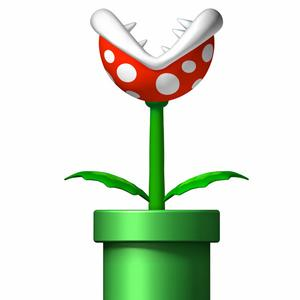
\includegraphics[width=\linewidth]{1-Esparcimiento/figs/plant}		
	\end{subfigure}
	\begin{subfigure}{.05\textwidth}%
		\vspace{-5cm}\caption{}\label{sfig:secondaty2}
		\end{subfigure}
	\begin{subfigure}{.43\textwidth} 
			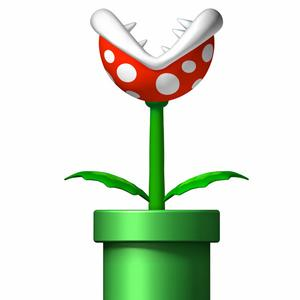
\includegraphics[width=\linewidth]{1-Esparcimiento/figs/plant}
	\end{subfigure}%
	\vspace*{-.25cm}
	\caption{The explanation of your figures. \blindtext}	\label{fig:Main}	
	\end{figure}	
				
\Blindtext
